\chapter{Bidirectional Texture Functions}
\label{chapter:stateOfArt}


\section{Acquisition}
\label{chapter:acquisition}

BTF acquisition is a non-trivial task as it requires a special acquisition setup. 
Only a few measurement systems \cite{star2004,schwartz,dana,Kaleidoscope,Koudelka,statistical_acq} exist, but as the interest in realistic material rendering using BTFs is growing, measurement systems are developing.
In this chapter we will review how in general BTF data acquisition is done, which post-processing steps are made, and advantages and disadvantages of existing measurement systems are discussed. 
We will also review publicly available BTF datasets.

\subsection{General Acquisition Methods}
\label{section:General_acquisition}	
All the mentioned BTF acquisition systems share the same idea in the data acquisition, i.e. capturing the appearance of a flat square slice of the material surface under varying light and camera directions.
The material surface is usually sampled over a hemisphere above the material slice, as shown in Figure \ref{fig:acquisition_example}.
Depending on the material's reflectance properties the sampling distribution may vary, e.g. the sampling distribution can be dense in regions where specular peaks in the light reflection occur. 
Then, if needed, a uniform distribution can be calculated in a post-processing step using interpolation \cite{haindl_visual}.

Digital cameras are used as capturing devices. Depending on the setup the number of cameras can vary.
 If there is only one camera \cite{star2004,statistical_acq,dana}, it usually moves on a robotic arm or rail-trail system around the hemisphere above the sample \cite{star2004}. 
 The advantage of this approach is that it is less expensive and can suit low-budget applications.
The disadvantage however is the positioning errors that can arise, which influence the overall measurement error. 
Depending on the application, light sources can be fixed or moveable.

There are approaches which do not involve camera and light source movement at all.
Schwartz et al. \cite{schwartz} developed a novel measurement system which uses a dense array of 151 cameras, which are uniformly placed on a hemispherical structure.
Flashes of the cameras are used as light sources. Such a setup provide a high angular and spatial resolution.

Ngan et al. \cite{statistical_acq} made a setup which does not involve camera movement by placing the planar slices of the material in the form of a pyramid.
Thus, such setup captures the material appearance for 13 different camera views at once. Light directions are sampled by a manually-moved electronic flash.
The disadvantage of this setup is that it provides sparse angular resolution, but depending on the application such an approach can be plausible.
For example, a material which does not exhibit high illumination changes can be sampled sparsely to reduce the amount of redundant data.

The material sample is commonly a flat and squared slice, which is placed on the holder plate. To conduct automatic post-processing borderline markers are placed on the holder.
Those markers provide the important information for further post-processing steps such as image rectification and registration.


\begin{figure}[h]
 \centering
 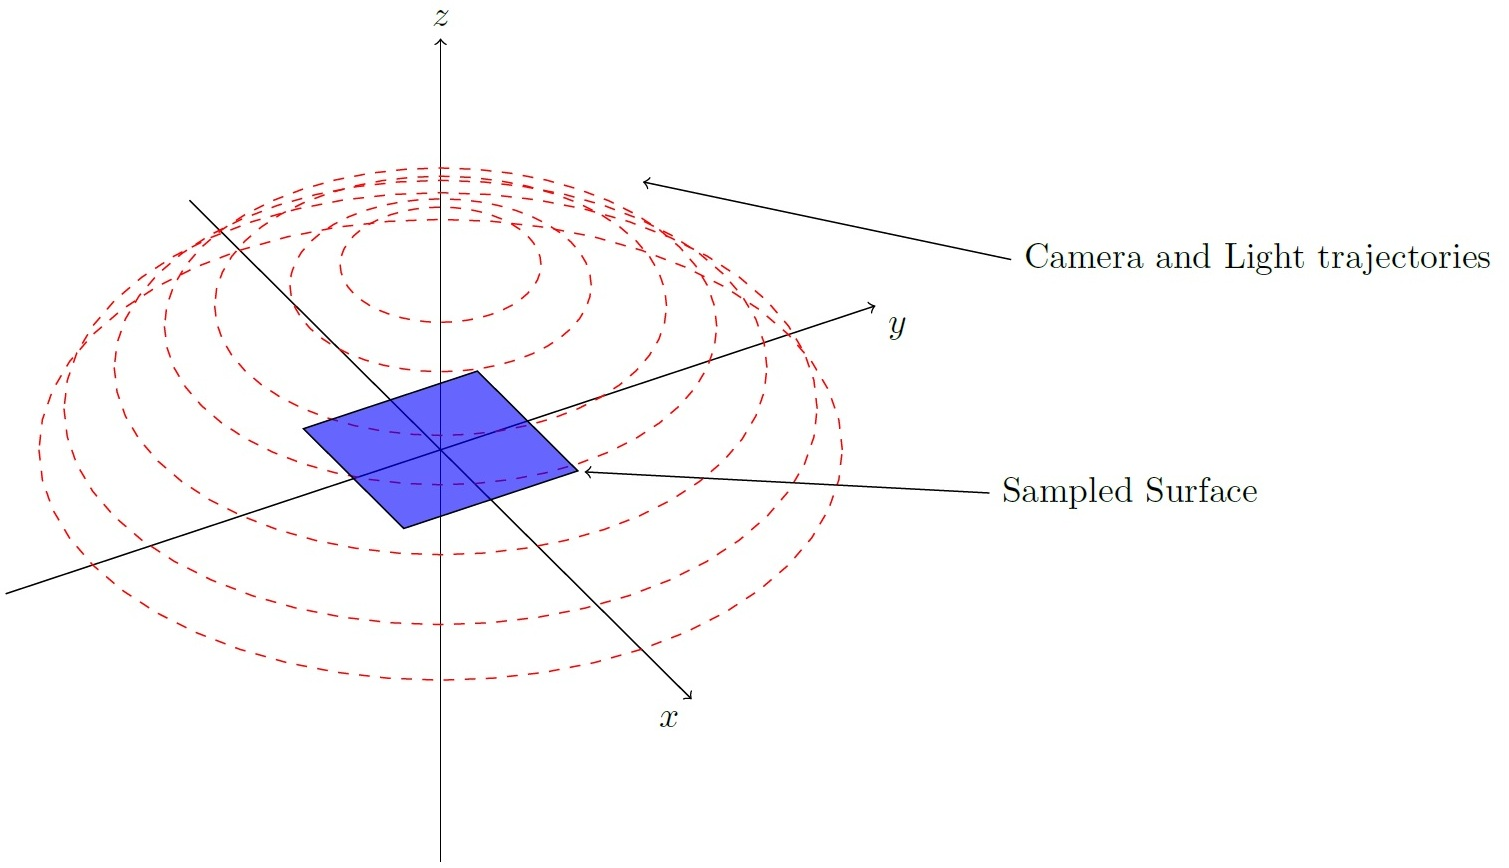
\includegraphics[width=1.0\textwidth]{figures/acquisition}
 \caption[Example of BTF measurement] {
 	{\bf Example of BTF measurement.}

	Camera and light positions share the same trajectories.
	Red dashed circles are the sample positions on the hemisphere. }
 \label{fig:acquisition_example}
\end{figure}

\subsection{Post-processing}
\label{section:Post_processing_acquisition}	
After the measurement is done, the raw data has to be further post-processed, because typically such  data is not ready for compression.
Raw data consists of a set of images that are not aligned with each other and are not mutually registered.

When these raw images are obtained under different camera angles $(\theta,\phi)$ they are perspectively distorted \cite{sattler-2003-efficient}.
Thus, all sample images have to be aligned with each other and spatially registered to be further used.
Firstly, borderline markers that were placed around the material sample on the holder plate aid the automatic detection of the material slice.
Then, after the material slices are detected and cropped, they are ready for mutual alignment. This process is called  \emph{rectification}. 
\emph{Rectification} is a process which involves projecting all sample images onto the plane which is defined by the frontal view, e.g. $(\theta _{o} =0,\phi _{o}=0)$.
In other words, all normals of the sample images have to be aligned with their corresponding camera directions, i.e. as if all sample images were taken from frontal view $(\theta =0,\phi=0)$.
The last step is image \emph{registration}, a process of getting pixel-to-pixel correspondence between the images.
Finally all images have to be scaled to an equal resolution.


Even after the proper rectification and registering of the measured data, registration errors can still be present between individual camera directions \cite{haindl_visual}. 
 This happens due to structural occlusion of the material surface. Because of such self-occlusion some geometries structures are not captured by certain camera directions.
 That is why even after rectification images captured from completely different directions are not correctly aligned
 registration errors can also be caused by both inaccurate camera and material sample positions happened during the measurement processes.


If needed, further processing steps can be done, for instance \emph{linear edger blending} to reduce tiling artifacts \cite{sattler-2003-efficient}.
Also, typical image processing steps may be employed, e.g. noise reduction filters. 


\subsection{Publicly Available BTF Datasets}
\label{section:Publicly_datasets}	

\begin{figure}[h]
 \centering
 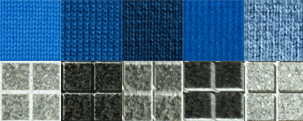
\includegraphics[width=1.0\textwidth]{figures/exampleBTF}
 \caption[Example of BTF measurement] {
 	{\bf BTF example of Bonn Database \cite{btfBonn}.}

	Example how BTF catches rich appearance of the material due to dependencies on light and camera directions. 
	Upper row is a knitted wool, lower is a graved granite stone.}
 \label{fig:exampleBTF}
\end{figure}


The accurate rendering of the material surface highly depends on the quality of the acquired data, especially for BTFs.
There are several properties that are vital for reproducing high quality rendering results.
 BTF datasets can be distinguished by how well image post-processing were done and how good spatial and angular resolutions are.

 
A pioneer in the BTF acquisition was Dana  \emph{et. al.} \cite{curetDataBase}, who measured 61 materials with fixed lighting and a moving camera aided by a robotic arm. 
This procedure resulted in a set of images, which can be seen as a subset of a BTF, which is called surface light field (SLF), see Chapter \ref{section:slf}.
Dana  \emph{et. al.} \emph{CUReT} database is publicly available \cite{curetDataBase}.
For each measured surface Dana  \emph{et. al.} used 205 different combinations of camera and light directions, which resulted in relatively sparse angular resolution.
These datasets are not rectified, but  the authors provide image coordinates to enable rectification. 
 Because of these limitations such BTF dataset are usually used for computer vision purposes, i.e. texture classification  \cite{haindl_visual}.

Based on this BTF measurement system,  Bonn University created their own measuring system \cite{sattler-2003-efficient}.
 The main difference of this system is that the camera moves on a semi-circle rail around the material sample.
Such a setup provides spatially rectificated and mutually registered data, with reasonable angular and spatial resolutions. 
Datasets of the Bonn University \cite{btfBonn} are publicly available and are used in this thesis.


 Consider Figure \ref{fig:exampleBTF}, which illustrates sample materials from the Bonn database.
The measured surface is being fixed all the time on the sampler holder as shown in Figure \ref{fig:acquisition_example}. 
For each light position, a camera takes a shot of the material while moving from point to point on the hemisphere.
Bonn University datasets have the same trajectory for camera and light positions, i.e. 81 positions on the hemisphere, which resulted in $81\times81=6561$ number of acquired images.
After that the sample images were rectificated and registered, resulting in a set of images with a spatial resolution of $256\times256$.
Typically, the size of one uncompressed BTF is around $1.2$ Gb.



\section{Data Representations}
\label{chapter:representations}




Before doing any further operations on the acquired BTF data it is important to chose a suitable representation for the data.
A suitable presentation can influence the final quality of the BTF rendering and the compression ratio enormously.
\subsection{Texture Representation}
\label{chapter:texture_repr}

 The first straightforward representation as a set of textures can mathematically represented as

{\centering $\,\,\,\,\,\,\,BTF_{Texture}=\left \{I_{(\theta_{i} ,\phi_{i},\theta_{o} ,\phi_{o}) }  \mid  (\theta_{i},\phi_{i},\theta_{o} ,\phi_{o})\in M \right \}$\\}


where $M$ denotes a set of images $I_{(\theta_{i} ,\phi_{i},\theta_{o} ,\phi_{o})}$ measured for different light and camera directions $(i,o)$ accordingly.

Basically, $BTF_{Texture}$ is used for compression methods that do their analysis on the whole sample plane.

\subsection{ABRDF Representation}
\label{chapter:abrdf_repr}

 ABRDF (Chapter \ref{section:brdf}) representation is a set of ABRDFs, one for each sample position of the material plane.
 In this case it is called \emph{apparent}, 
 because BTF includes effects such as self-occlusions and sub-surface scattering which violate two basic properties of a BRDF, i.e. \emph{energy conservation} and \emph{reciprocity}.
 
 {\centering $\,\,\,\,\,\,\,\,\,\,\,\,\,\,\,\,BTF_{ABRDF}=\left \{P_{(x) } \,\,\,\,\,\,\,\,\,\,\,\,\,\,\,\,\,\,\mid  (x)\in I_{(\theta_{i} ,\phi_{i},\theta_{o} ,\phi_{o})}\subset \mathbb{N}^{2}\right \}$ \\}
 
 $BTF_{ABRDF}$ denotes a set of $P_{(x)}$ images, i.e. ABRDF for spatial position $x$.


 $BTF_{ABRDF}$ representation allows better pixel-to-pixel comparisons, which can give a big advantage for methods that employ pixel-wise compression, e.g. BRDF based models.

Also, such arrangement provides images with lower variance \cite{haindl}, which can allow better compression results in certain scenarios, e.g. when the material surface is not smooth.

 
\section{BTF Compression Methods}
\label{chapter:compression_methods}



 A measured BTF consists of thousands of images, which require lots of storage space.
In the Bonn  Database \cite{btfBonn} a BTF consists of 8-bit PNG images with a resolution of $256\times256$ sampled for $81\times81$ different camera and light directions.
 An uncompressed BTF is approximately $1.2$ GB in size.
 To render a scene with several BTFs and to achieve an acceptable frame-rate becomes practically impossible, especially for low-end hardware.
 Also, as we intent to render BTFs in a web-browser, the data has to be transferred from the server to the client, which means the compact representation of the BTF is of utmost importance.
 For our scenario it is important to chose a compression method, that allows for real-time decompression, high compression rates while preserving good quality, and separability of compressed BTF data.
 Separability is needed for real-time streaming in a web-browser.  
 As the data is streamed in small chunks, partial data has to be renderable to produce a preview of the BTF.

There are different methods for BTF compression. Those methods can be categorized as follows:

\begin{itemize}
  \item \emph{Analytic methods} represent BTFs through analytic BRDF models. 
These analytic BRDF models are fitted separately to each texel of the BTF. These functions only have a few parameters, thus real-time performance is easily achieved.
However, these groups of methods can suffer from decreased rendering quality \cite{haindl}. In addition, it is hard to change parameters in order to control the visual quality. (See Chapter  \ref{section:analytic_methods}).
   \item \emph{Statistical methods}, which belong to methods that reduce dimensionality based on  statistics, for instance based a linear basis decompression method such as PCA (Principal component analysis). 
    PCA based methods are frequently used, because its parameters directly correspond to the trade-off between compression ratio and reconstruction quality.
    Also, PCA is frequently the basis for some more sophisticated methods \cite{webglbtfstreaming}. (See Chapter \ref{section:stat_methods}.)
   \item \emph{Probabilistic models} can achieve high compression rates, but the resulted image quality is generally only suitable for flat surfaces.
  Additionally, the implementation on a GPU is problematic. (See Chapter \ref{section:prob_methods}.)
 \end{itemize}



 \subsection{Analytic methods}
\label{section:analytic_methods}	
 This group of methods take advantage of the ABRDF representation of a BTF. 
 There is a large number of techniques which allow for a compact representation of BRDFs, which in general can also be applied to ABRDFs.
 Each texel of a BTF, i.e. spatial position on the surface are represented as a ABRDF. Each of these ABRDFs can be modeled and compressed by any BRDF model.
 
One of the possible ways to model ABRDF is to use \emph{Polynomial Texture  Mapping} (PTM).
Malzbender  \emph{et. al.} \cite{PTM} used this approach which allows for high compression rates and good quality. 
However, PTM requires to compute specular and diffuse effects separately. 
The PTM model assumes that the input surface is either diffuse or their specular contribution has been separated beforehand.
For BTFs it can be difficult to separate specular highlights \cite{haindl}.

Haindl  \emph{et. al.} \cite{haindl} applied PTM on Reflectance Fields (PTM RF)

{\centering$R_{o}(r,i)\approx a_{0}(r)u_{x}^2+a_{1}(r)u_{y}^2+a_{2}(r)u_{x}u_{y}+a_{3}(r)u_{x}+a_{4}(r)u_{y}+a_{5}(r)$\\}

 where $R_{o}$ is the approximated RF for a fixed camera direction $o$ and $u_{x},u_{y}$ are projections of the normalized light vector into the local coordinate system $r=(x,y)$.
 The set of all possible $R_{o}$ is the number of all camera positions, i.e. $n_{o}$. 
 Coefficients $a_{p}$ are fitted by the use of \emph{singular value decomposition} (SVD) for each $R_{o}$ and parameters are stored as a spatial map referred to as a PTM.
 
  This method enables fast rendering and is generally suited for smooth material surfaces.
  However, Malzbender  \emph{et. al.} \cite{PTM} claim that this method produces considerable errors for grazing angles. 

 
 Another model which produces slightly better visual quality is the polynomial extension of the one-lobe Lafortune model (PLM) \cite{haindl}.


{\centering$Y_{o} (r,i) = \rho_{o,r}(C_{o,r,x}u_{x}+C_{o,r,y}u_{y}+C_{o,r,z}u_{z})_{ }^{n_{o,r}}$\\}

where $w_{i}(\theta_{i}, \phi_{i})=[u_{1},u_{2},u_{3}]^{T}$ is the unit vector pointing from surface to light.
Parameters $\rho,C_{x},C_{y},C_{z},n$ can be computed with a Levenberg-Marquardt non-linear optimisation algorithm \cite{plm}. 
 Filip and Haindl \cite{plm} claim that the one-lobe Lafortune model produces unsatisfactory results for complex ABRDFs.
 Thus, the polynomial extension of the one-lobe Lafortune was introduced (PLM RF):

{\centering$R_{o}(r,i)\approx  \sum_{j=0}^{n} a_{r,o,i,j}Y_{o}(r,i)^j$\\}



PLM RF solves the problem of bad quality for grazing angles and improves the rendering quality compared to PTM RF.
However, statistical based methods produce even better quality compared to above methods but with lower compression rates \cite{haindl}.



  \subsection{Statistical methods}
\label{section:stat_methods}
This group of methods is mostly based on a dimensionality reduction of the data, while preserving the most important information.
The goal of dimensional reduction is to find a new basis which would represent the data with less dimensions and at the same time preserving the important features of the original data.
 The size of the data with the new basis will be decreased.

One of the popular methods used for BTF compression belongs to this group, i.e. \emph{Principal component analysis} (PCA) \cite{Bishop,schneider2004,haindl,webglbtfstreaming,sattler-2003-efficient,mueller-2003-compression,gpu_gems}.
PCA is a linear transformation of the data to a new basis, where each new coordinate (variable) is called a \emph{principal component} \cite{Bishop}.
All new coordinates are mutually orthogonal, i.e. uncorrelated. Components are sorted by decreasing variance, i.e. the first component posses the greatest variance compared to other components. 
 The last components which hold small variations are discarded, because they do not contribute important information.

PCA is a popular approach for compressing BTF. 
Firstly, PCA allows for a strong correspondence between the number of components and the decompression error.
 The correspondence lies in the amount of components used.
 The more components used the better the decompression error is, and vise-verse, a smaller number of components gives better compression ratio, but worse decompression error.
 This allows for an easy  regulation of the trade-off between rendering quality and  compression ratio.
Secondly, a reasonable compression ratio along with a low decompression error can be achieved, e.g. a compression ratio of $1:100$ with an average decompression error of 2\%- 4\% \cite{schneider2004,haindl}.
Thirdly, PCA is suitable for real-time decompression on average GPUs \cite{schneider2004,haindl}. 
It is suitable, because decompression of a single pixel does not depend on other pixels.
 Computation of a single pixel for PCA decompression on the GPU is done by means of linear combinations of estimated PCA parameters, so the speed of decompression depends on the number of components used.
 
 There exist different methods based on PCA, for instance PCA \emph{Reflactance Field} (RF), PCA BTF and local PCA (LPCA) \cite{sattler-2003-efficient,schneider2004,mueller-2003-compression, haindl}.
 Sattler \emph{et. al.} \cite{sattler-2003-efficient} developed PCA RF. 
 This method ensures a pixel position coherence, by employing PCA per camera direction. 
 The advantage is that on average 8 components are enough to get good results with decompression errors around 2\%- 4\%.
 On the other hand, PCA BTF, which does PCA on all camera directions at once, requires on average 41 components \cite{haindl}.
 M{\"u}ller  \emph{et. al.} \cite{schneider2004} improved PCA BTF by exploiting vector quantization techniques and applying PCA on the resulted clusters.
Local PCA (LPCA) requires 19 components on average \cite{haindl}.
 Even though the compression ratio of PCA RF is lower than PCA BTF and LPCA, it is less computational demanding.


In general, any PCA method is suitable for streaming, as it is possible to stream components separately and progressively enhance the rendering quality. 



 \subsection{Probabilistic models}
\label{section:prob_methods}

Compression methods based on probabilistic models \cite{car_model,gmrf_model,haindl}
 provide much higher compression rates than most others methods and allow for a seamless enlargement of textures of any size \cite{haindl}. 
Usual compression ratios achieved by such models are $1:6-8\times 10^{4}$.
The visual quality of the rendered results are best suited for smooth materials, while materials with high frequencies can appear flat using probabilistic methods \cite{haindl}.
Also, these type of models can be problematic for implementation on low-end GPUs. 
The problem arise in shaders, when probabilistic models require information of spatial neighbours to synthesize the texture \cite{gmrf_model,haindl}.
Even though solutions exists to handle this problem, e.g. take advantage of Framebuffer Objects, which allow access to previously rendered results \cite{haindl},
these solutions are time-consuming for low-end GPUs.





